% This is samplepaper.tex, a sample chapter demonstrating the
% LLNCS macro package for Springer Computer Science proceedings;
% Version 2.20 of 2017/10/04
%
\documentclass[runningheads]{llncs}
%
\usepackage{graphicx}
% Used for displaying a sample figure. If possible, figure files should
% be included in EPS format.
%
% If you use the hyperref package, please uncomment the following line
% to display URLs in blue roman font according to Springer's eBook style:
% \renewcommand\UrlFont{\color{blue}\rmfamily}

\begin{document}
%
\title{The best work\thanks{Degree in Software Engineering, University of Oviedo}}
%
%\titlerunning{Abbreviated paper title}
% If the paper title is too long for the running head, you can set
% an abbreviated paper title here
%
\author{Arroni del Riego, Sergio\orcidID{276341} \and
Alex\orcidID{1111-2222-3333-4444} \and
Manu\orcidID{2222--3333-4444-5555}}
%
\authorrunning{Arroni del Riego, Sergio \and Alex \and Manu}
% First names are abbreviated in the running head.
% If there are more than two authors, 'et al.' is used.
%
\institute{Oviedo University, Oviedo Asturias, Spain\\
\url{https://uniovi.es}}
%
\maketitle              % typeset the header of the contribution
%
\begin{abstract}
The abstract should briefly summarize the contents of the paper in
15--250 words.

\keywords{A*  \and PEA* \and Search \and heuristic \and 8-puzzle.}
\end{abstract}
%
%
%
\section{Introduction}
In this section, we will introduce the subject to be dealt with as well 
as a brief description of the rest of the sections of the work.

\subsection{Description of the topic to be addressed}
In this work we are going to apply the algorithm A* and PEA* to the 8-puzzle problem, 
for this we are going to use different heuristics, 
one of these heuristics is the one we propose in this work, 
which we call "The most humble first" or MHF. 

\subsection{Description of the sections of the work}
In the following points we will discuss:
\begin{enumerate}
\setcounter{enumi}{1}
\item Description of the 8-puzzle problem, in this section we will detail how the problem in question works.
\item Description of the algorithms involved in the work, in this section we will explain in detail how the algorithms used work, as well as a brief state of the art of them.
\item Application of the algorithms to the 8-puzzle problem, we will explain the approach we have taken to the 8-puzzle problem, as well as the heuristics to be used, including the one we propose in this work.
\item Experimentation, we will compare different heuristics, as well as the one proposed in this wok.
\item Conclusion, here we will give our critical opinion on this application of the algorithm.
\end{enumerate}

\section{The 8-puzzle problem}
The 8-puzzle problem is well known and used for the study of search algorithms, informed or uninformed, 
generally of the second type, i.e., they also include the study of various heuristics that try to reach 
the objective state in the optimal way. However, heuristics can be applied simply with the intention to 
analyze it without the need for it to be good.

\subsection{Description of problem}
It is actually a concrete example of the n-puzzle problem, which is used because it is simple to understand 
at this size.

So, for this particular example, we have a 3x3 board where 8 of the cells are filled with all the numbers 
from 1 to 8 while one remains empty. This will be the one to which we have to move the cells in order to reach 
the desired final state.

There are 4 possible movements, displacement of a cell to its adjacent cell located in the north, south, east 
or west as long as the cell is empty in one of the locations.

The cost of each movement is 1, and the goal is to reach the target state by adding as few movements as possible 
and, therefore, achieving the lowest cost.

\subsection{Classic methods of resolution}
As I said at the beginning, the algorithms that can be used to solve this problem can be informed, such as algorithms 
A*, PEA*, IDA*, and not informed such as DFID, BFS....

We will study the application of the A* and PEA* algorithms with heuristics having different characteristics.

\begin{figure}
\centering
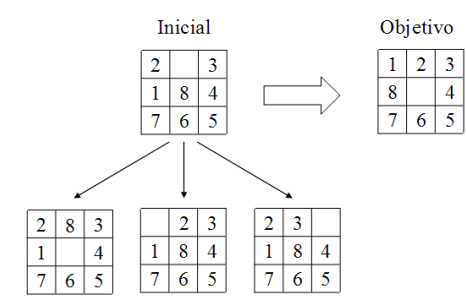
\includegraphics[width=0.65\textwidth]{8puzzle.png}
\caption{Figure showing the starting point, the objective and the stages we went through to achieve it.} \label{fig1}
\end{figure}

\section{The search algorithms}
In this section, we will discuss about search algorithms, doing a distincion between uninformed and informed search algorithms.
The uninformed algorithms that we will discuss are: Best First (\(BF\)).
The informed algorithms that we will discuss are: A* and PEA*.

\subsection{Best first search (\(BF\))}
The uninformed search algorithms are those thay do not use any information about the problem, they just expand the next node in the frontier.
The most important thing that differentiates the various uninformed algorithms is the method they use to expand the next node in the frontier.
Hereafter, we will trate the Best First (\(BF\)) search algorithm.

We will start with the "Best First" (\(BF\)) search algorithm \cite{algorithms}, which is the basis of informed search algorithms, such as \(A^*\).
\(BF\) is based on the idea of idea of expanding the node with the lowest cost. The cost of a node is calculated by the heuristic function \(h(n)\) used. \\
In the \(BF\) algorithm, we have two list, the list "open" that this list contains the nodes that are not expanded yet, and the list "closed" that contains the nodes that are expanded:
\begin{enumerate}
\item Initialises the "open" list with the start node.
\item Initialises the "closed" list with the empty list.
\item While the "open" list is not empty:
\begin{enumerate}
\item Select the node with the lowest cost, following the given \(h(n)\), in the "open" list and remove it from the "open" list.
\item If the node is the goal, stop.
\item If not, add the node to the "closed" list and expand its children.
\item For each child:
\begin{enumerate}
\item If the child is in the "closed" list, do nothing.
\item If the child is not in the "open" list, add it.
\item If the child is in the "open" list, but the path to the child is better than the previous path, replace the child in the "open" list with the new child.
\end{enumerate}
\end{enumerate}
\item Return to Step 3.
\end{enumerate}
You can see a more detailed description and a implementation of the algorithm in Russell's and Norvig's book \cite{algorithms_2}.

\subsection{\(A^*\)}

The informed search algorithms are those that use the any information about the problem to expand the next node in the frontier.\\
The \(A^*\) algorithm is a variation of the \(BF\) algorithm, this was proposed by Peter E. Hart, Nils J. Nilsson and Bertram Raphael in their work in 1968 \cite{algorithms_3}.\\
In \(A^*\), use a function \(f\) to evaluate the nodes, this function in \(A^*\) is representate by \(f^*(n)\) and this is the cost of the shortest path from initial to \(n\) conditional on passing through \(n\).
The function \(f^*(n)\) (where n is any node) is defined as equation \ref{eqn:a*}:

\begin{equation}\label{eqn:a*}
f^*(n) = g^*(n) + h^*(n)
\end{equation}

Where \(g^*(n)\) is the cost of the path from the initial node to the node \(n\), and \(h*(n)\) is the heuristic function that estimates the cost of the path from the node \(n\) to the goal node, you can see this function in more detail in Nilsson's book "Principles of artificial intelligence" \cite{algorithms_4}.
In A* we talk about f*, g* and h*, but in most cases these are only estimates because it is very complicated for complex problems to know the exact values, if we knew them the algorithm would go straight to the goal. Instead we use the estimates f, g and h, so the function would be as we can see in equation \ref{eqn:a_2}:

\begin{equation}\label{eqn:a_2}
f(n) = g(n) + h(n)
\end{equation}

The \(A^*\) algorithm is as follows, we have two list, the list "open" that this list contains the nodes that are not expanded yet, and the list "closed" that contains the nodes that are expanded:

\begin{enumerate}
\item Initialises the "open" list with the start node.
\item Initialises the "closed" list with the empty list.
\item While the "open" list is not empty:
\begin{enumerate}
\item Select the node with the lowest cost, you can se the equation in \ref{eqn:a*}, in the "open" list and remove it from the "open" list.
\item If the node is the goal, stop.
\item If not, add the node to the "closed" list and expand its children.
\item For each child:
\begin{enumerate}
\item If the child is in the "closed" list, do nothing.
\item If the child is not in the "open" list, add it.
\item If the child is in the "open" list, but the \(f(child)\) is better than the previous path, replace the child in the "open" list with the new child.
\end{enumerate}
\end{enumerate}
\item Return to Step 3.
\end{enumerate}

One problem that have the \(A^*\) algorithm is that it can be very slow, because it can expand a lot of nodes, and this can be a problem if the problem has a lot of nodes. To solve this problem, we can use the PEA* algorithm.\\
If you want to see a more detailed description and a implementation of the algorithm, you can see Russell's and Norvig's book \cite{algorithms_2}.

\subsection{\(PEA^*\)}
The \(PEA^*\) algorithm is a variation of the \(A^*\) algorithm, in fact it is faster than the base algorithm \(A^*\).
\(PEA^*\) is a not admitted algorithm, this means that it is not guaranteed to find the optimal solution, but it is very fast and it is very useful in practice.
The \(PEA^*\) algorithm have a function, very similar to the \(A^*\) function, but it is not the same, this function is called \(f_{PEA}^*(n)\) and is defined in equation \ref{eqn:pea*}:

\begin{equation}\label{eqn:pea*}
f_{PEA}^*(n) = g^*(n) + h^*(n) * (1 + \epsilon)
\end{equation}

Where \(g^*(n)\) is the cost of the path from the initial node to the node \(n\), 
\(h*(n)\) is the heuristic function that estimates the cost of the path from the node \(n\) to the goal node and 
\(\epsilon\) is a constant that is used to control the expansion of the nodes.\\
You can see this algorithm in more detail in Maria Rita's tesis \cite{algorithms_5}.

\section{Application of the A* and \(PEA^*\) algorithms to the 8-puzzle problem}
The two algorithms that we are going to study are informed, i.e., we are facing a heuristic search and, therefore, we have to apply a heuristic to reach the solution, 
we have to apply a heuristic to reach the solution. The state space of this problem is defined by 
the set of possible combinations on the board, i.e. the location of all the tiles.

We will apply the same heuristics to both algorithms. They are the following:
\begin{enumerate}
    \item h1(n): number of tiles that are out of place. Easy to perform, but does not provide the best possible results. Monotone.
    \item h2(n): sum of orthogonal distances from each tile to its final position. Effective for short problems giving the best solutions. Monotone.
    \item h3(n): 2*number of tiles at orthogonal distance 2 from their final position
\end{enumerate}

\section{Experimental study}
TODO

\section{Conclusions}
TODO

\section{DE AQUI PARA ABAJO = BASURA, LO DEJO DE EJEMPLO}
Please note that the first paragraph of a section or subsection is
not indented. The first paragraph that follows a table, figure,
equation etc. does not need an indent, either.

Subsequent paragraphs, however, are indented.

\subsubsection{Sample Heading (Third Level)} Only two levels of
headings should be numbered. Lower level headings remain unnumbered;
they are formatted as run-in headings.

\paragraph{Sample Heading (Fourth Level)}
The contribution should contain no more than four levels of
headings. Table~\ref{tab1} gives a summary of all heading levels.

\begin{table}
\caption{Table captions should be placed above the
tables.}\label{tab1}
\begin{tabular}{|l|l|l|}
\hline
Heading level &  Example & Font size and style\\
\hline
Title (centered) &  {\Large\bfseries Lecture Notes} & 14 point, bold\\
1st-level heading &  {\large\bfseries 1 Introduction} & 12 point, bold\\
2nd-level heading & {\bfseries 2.1 Printing Area} & 10 point, bold\\
3rd-level heading & {\bfseries Run-in Heading in Bold.} Text follows & 10 point, bold\\
4th-level heading & {\itshape Lowest Level Heading.} Text follows & 10 point, italic\\
\hline
\end{tabular}
\end{table}


\noindent Displayed equations are centered and set on a separate
line.
\begin{equation}
x + y = z
\end{equation}
Please try to avoid rasterized images for line-art diagrams and
schemas. Whenever possible, use vector graphics instead (see
Fig.~\ref{fig1}).

\begin{theorem}
This is a sample theorem. The run-in heading is set in bold, while
the following text appears in italics. Definitions, lemmas,
propositions, and corollaries are styled the same way.
\end{theorem}
%
% the environments 'definition', 'lemma', 'proposition', 'corollary',
% 'remark', and 'example' are defined in the LLNCS documentclass as well.
%
\begin{proof}
Proofs, examples, and remarks have the initial word in italics,
while the following text appears in normal font.
\end{proof}
For citations of references, we prefer the use of square brackets
and consecutive numbers. Citations using labels or the author/year
convention are also acceptable. The following bibliography provides
a sample reference list with entries for journal
\cite{BFS}
%
% ---- Bibliography ----
%
% BibTeX users should specify bibliography style 'splncs04'.
% References will then be sorted and formatted in the correct style.
%
% \bibliographystyle{splncs04}
% \bibliography{mybibliography}
%

\bibliography{refs} 
\bibliographystyle{ieeetr} 

\end{document}
